\section{Pruebas funcionales}
\label{sec:pruebas_funcionales}

Las pruebas funcionales verifican que cada componente del sistema se comporta
conforme a su especificación. Se ejecutaron sobre el escenario Docker Compose
(reproducible en cualquier equipo) con cuatro fuentes de prueba FFmpeg generando
señal sintética a 1920$\times$1080@25\,fps.

La tabla~\ref{tab:hardware} recoge las especificaciones del equipo utilizado.

\begin{table}[H]
  \centering
  \caption{Especificaciones del equipo empleado en las pruebas.}
  \label{tab:hardware}
  \begin{tabular}{|l|l|}
    \hline
    \textbf{Componente} & \textbf{Especificación} \\
    \hline
    CPU      & Intel Core i7-8750H @ 2,20\,GHz (6 núcleos / 12 hilos) \\
    RAM      & 16\,GB DDR4 2666\,MHz \\
    Sistema  & Ubuntu 22.04 LTS (kernel 6.8) \\
    Docker   & Docker Engine 26.1 / Compose v2.27 \\
    Red      & Loopback gigabit (escenario Docker); WiFi 5\,GHz (escenario 2\,PCs) \\
    \hline
  \end{tabular}
\end{table}

\subsection{Conmutación de fuentes y composites}

Se ejecutó una secuencia de 20 cambios de fuente (Cut y Trans) y 10 cambios de
composite alternando entre los modos \texttt{fs}, \texttt{pip}, \texttt{sbs} y
\texttt{lec}. En todos los casos:

\begin{itemize}
  \item El cambio fue efectivo en el siguiente fotograma tras la pulsación del botón.
  \item El registro \texttt{.jsonl} generó una entrada de tipo \texttt{CHANGE} con
        la marca de tiempo correcta y el nuevo estado de \texttt{video} y
        \texttt{composite}.
  \item El botón Retake restauró el estado previo sin generar artefactos visuales.
\end{itemize}

\begin{table}[H]
  \centering
  \caption{Resultados de las pruebas de conmutación.}
  \label{tab:pruebas_conmutacion}
  \begin{tabular}{|l|c|c|}
    \hline
    \textbf{Prueba} & \textbf{Intentos} & \textbf{Resultado} \\
    \hline
    Cut cam $\rightarrow$ cam            & 20 & \textbf{20/20} correctos \\
    Trans composite $\rightarrow$ composite & 10 & \textbf{10/10} correctos \\
    Retake tras corte erróneo           & 5  & \textbf{5/5} correctos \\
    Cambio de composite durante Trans   & 3  & \textbf{3/3} sin artefactos \\
    \hline
  \end{tabular}
\end{table}

\subsection{Stream blanker}

Se verificaron las tres transiciones de estado del stream blanker:
LIVE\,$\rightarrow$\,PAUSE, PAUSE\,$\rightarrow$\,NOSTREAM y
NOSTREAM\,$\rightarrow$\,LIVE. En cada caso se comprobó visualmente que el puerto
15000 emitía el vídeo alternativo correcto y que el puerto 11000 (mezcla bruta)
permanecía inalterado, confirmando el aislamiento entre la señal de grabación y la
señal de distribución pública.

\subsection{Overlays y rotulación dinámica}

Se cargaron sucesivamente tres overlays PNG distintos y se introdujeron rótulos de
texto mediante los dos campos de rotulación simultánea. Las pruebas verificaron:

\begin{itemize}
  \item Fundido de entrada y salida (\textit{blend-in}/\textit{blend-out}) sin
        fotogramas corruptos.
  \item Actualización del texto con latencia inferior a un fotograma.
  \item Funcionamiento correcto del \textit{auto-off}: al realizar un corte de cámara
        con la opción activada, el overlay desapareció automáticamente sin
        intervención del operador.
  \item Recarga de recursos mediante el botón UPDATE sin interrumpir la señal.
\end{itemize}

\subsection{Sistema de telemetría}
\label{sec:prueba_telemetria}

Para verificar el correcto registro de eventos se ejecutó la siguiente secuencia
sobre el escenario Docker Compose:

\begin{enumerate}
  \item Cambio de fuente (cam1 $\rightarrow$ cam2).
  \item Cambio de composite (fs $\rightarrow$ pip).
  \item Activación de stream blanker PAUSE y vuelta a LIVE.
  \item Carga y descarga de overlay.
\end{enumerate}

Se accedió a la consola de administración de RabbitMQ
(\texttt{http://localhost:15672}) y se verificó que la cola \texttt{voctomix\_events}
contenía un mensaje por cada acción. La figura~\ref{fig:rabbitmq_placeholder}
muestra el aspecto esperado de la consola con mensajes en cola.

% ── Placeholder: captura real de la consola RabbitMQ ─────────────────────
\begin{figure}[H]
  \centering
  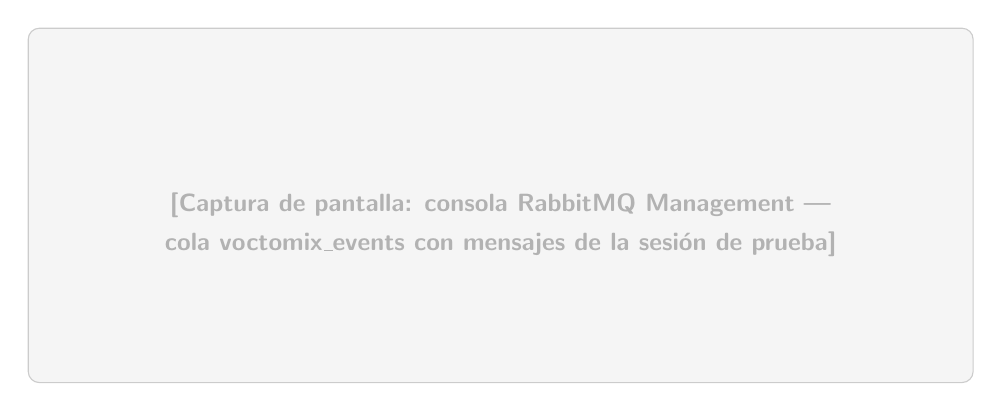
\begin{tikzpicture}
    \draw[rounded corners=4pt, fill=gray!8, draw=gray!40]
      (0,0) rectangle (12,4.5);
    \node[font=\sffamily\small\bfseries, text=gray!60] at (6,2.25)
      {[Captura de pantalla: consola RabbitMQ Management —};
    \node[font=\sffamily\small\bfseries, text=gray!60] at (6,1.75)
      {cola voctomix\_events con mensajes de la sesión de prueba]};
  \end{tikzpicture}
  \caption{Consola de administración RabbitMQ mostrando la cola
           \texttt{voctomix\_events} con los eventos registrados durante
           la sesión de prueba (captura pendiente de sustituir).}
  \label{fig:rabbitmq_placeholder}
\end{figure}

Se ejecutó también el script \texttt{rabbit\_consumer\_example.py} para volcar el
contenido de los mensajes y comprobar que la estructura JSON era correcta:

\begin{verbatim}
{"timestamp": "2025-03-28T20:14:32.105Z", "type": "CHANGE",
 "video": {"program": "cam2", "preview": "cam1"},
 "composite": "fs", "stream": "live",
 "performance": {"cpu": 34.2, "ram_pct": 8.7,
                 "bandwidth_mbps": 622.1}}
\end{verbatim}

\subsection{Validación del despliegue en Docker y Kubernetes}

En ambos escenarios contenerizados se verificó el arranque limpio del sistema
comprobando que todos los servicios alcanzaban el estado \textit{healthy}/\textit{ready}
antes de que la GUI intentara conectarse. La figura~\ref{fig:kubectl_pods} muestra
la salida de \texttt{kubectl get pods} con todos los contenedores en estado
\texttt{Running} y \texttt{Ready}.

% ── Placeholder: salida kubectl get pods ─────────────────────────────────
\begin{figure}[H]
  \centering
  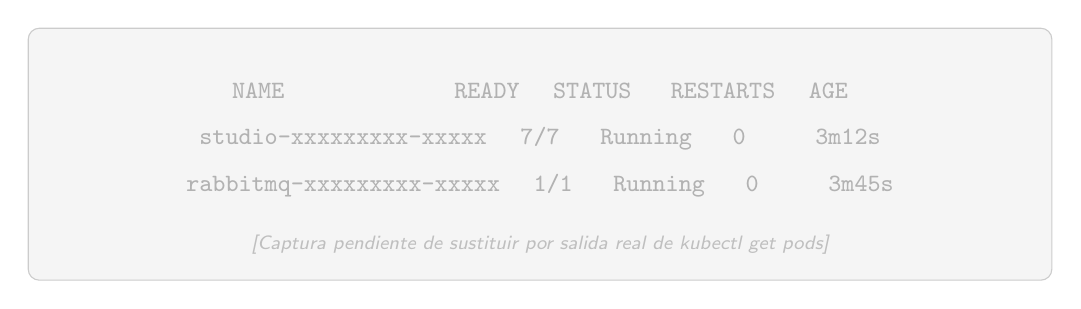
\begin{tikzpicture}
    \draw[rounded corners=4pt, fill=gray!8, draw=gray!40]
      (0,0) rectangle (13,3.2);
    \node[font=\ttfamily\small, text=gray!60] at (6.5,2.4)
      {NAME \quad\quad\quad\quad\quad\quad READY \; STATUS \quad RESTARTS \; AGE};
    \node[font=\ttfamily\small, text=gray!60] at (6.5,1.8)
      {studio-xxxxxxxxx-xxxxx \; 7/7 \;\; Running \;\; 0 \;\;\;\;\;\; 3m12s};
    \node[font=\ttfamily\small, text=gray!60] at (6.5,1.2)
      {rabbitmq-xxxxxxxxx-xxxxx \; 1/1 \;\; Running \;\; 0 \;\;\;\;\;\; 3m45s};
    \node[font=\sffamily\scriptsize\itshape, text=gray!50] at (6.5,0.45)
      {[Captura pendiente de sustituir por salida real de kubectl get pods]};
  \end{tikzpicture}
  \caption{Salida de \texttt{kubectl get pods} con todos los contenedores
           del sistema en estado \texttt{Running} y \texttt{Ready}
           (captura pendiente de sustituir).}
  \label{fig:kubectl_pods}
\end{figure}
